\subsection{実務上の考慮}

\subsubsection{インシデントと問題の予防}

インシデントや問題を予防するには、運用プロセス全体を可能な限り自動化し、試験を継続的に統合する必要がある。さらに、製品テレメトリを適切な分析技法と組み合わせ、問題を早期に検出する。

データは、アプリケーション層、オペレーティングシステム層、インフラ層など、製品スタックのすべての層から収集されるべきである。テレメトリは、問題の兆候を発見するだけでなく、問題源を特定するための基盤になる。

\subsubsection{運用リスク管理}

運用担当技術者は、可用性、拡張性、セキュリティ、個人情報漏えい、誤配備、容量不足、外部サービス停止など、多くのリスクを管理する。継続的リスク管理では、運用状態を常に監視し、リスクを検出したら自動的にアラートを出す。

何をアラートにするかは、製品責任者やソフトウェア技術者と相談して、リスク許容度を定める必要がある。すべての小さな変化で警報を出すと、警報疲れが起こる。逆に、重大な兆候を見逃すと、障害や事故につながる。

\subsubsection{ソフトウェアエンジニアリング運用の自動化}

現代の運用では、自動化が中心的役割を持つ。環境構築、ユーザアカウント作成、サーバ準備、実行時設定変更、配備、試験、デバッグ支援などを自動化できる。ソフトウェア技術者は、アプリケーション自動化と運用自動化を結びつけることで大きな効果を得る。

運用自動化の傾向は、複雑さを減らし、インフラ準備を速め、開発者へ運用サービススクリプトを提供し、アプリケーション定義、配備、試験作業を自動化する方向にある。

\par\smallskip
\begin{center}
\centering
\IfFileExists{assets/generated_figures/ch06/fig-ch06-11.png}{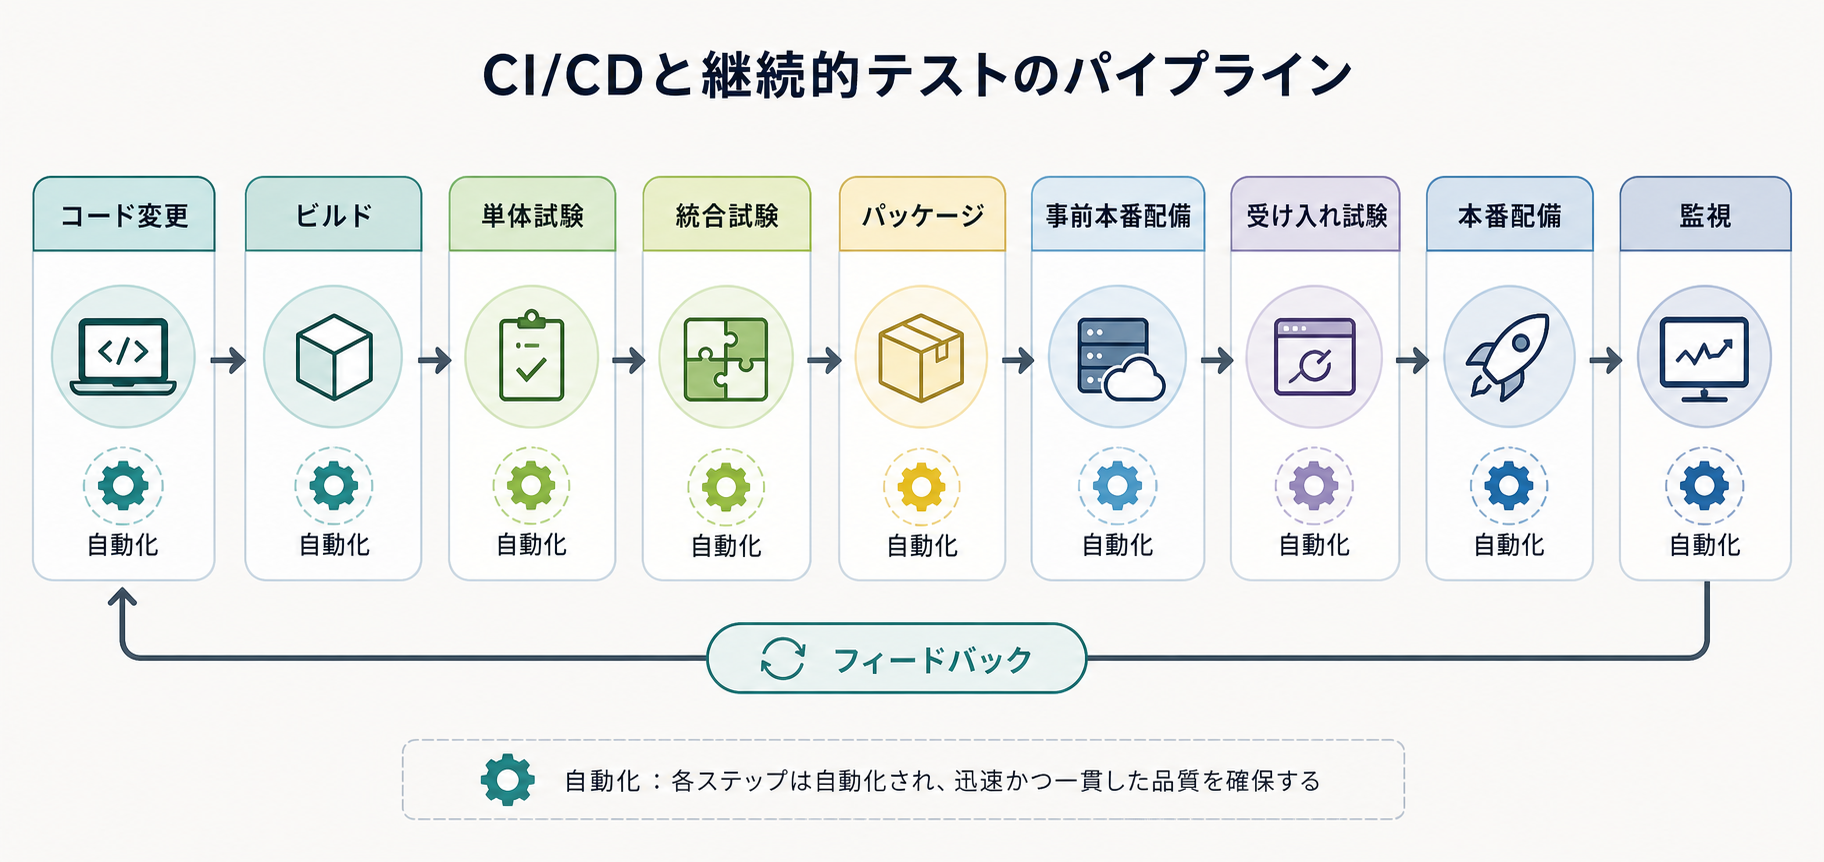
\includegraphics[width=0.96\linewidth]{assets/generated_figures/ch06/fig-ch06-11.png}}{\fbox{\parbox[c][48mm][c]{0.9\linewidth}{\centering 画像生成待ち\\CI/CDと継続的テストのパイプライン}}}
\par\smallskip
\refstepcounter{figure}\label{fig:ch06-11}図 \thefigure: CI/CDと継続的テストのパイプライン
\end{center}
図 \thefigure は、CI/CDと継続的テストのパイプラインを視覚的に整理したものである。
\par\smallskip

\subsubsection{小規模組織における運用}

小規模組織、とくに25人以下の非常に小さい組織では、大規模組織向けの標準をそのまま適用することが難しい。標準が要求する文書、役割、手順、監査が過大になることがある。この場合、小規模組織向けに調整されたISO/IEC 29110系列のような指針が有用である。

重要なのは、小規模であることを理由に運用を無視しないことである。むしろ、少人数だからこそ、自動化、標準化、簡潔な手順、明確な責任分担が重要になる。小規模組織では、最小限のSLA、バックアップ手順、インシデント対応、変更管理、監視ダッシュボードから始めるとよい。
